\section{Introduction}

\begin{figure*}[!t]
  \centering
  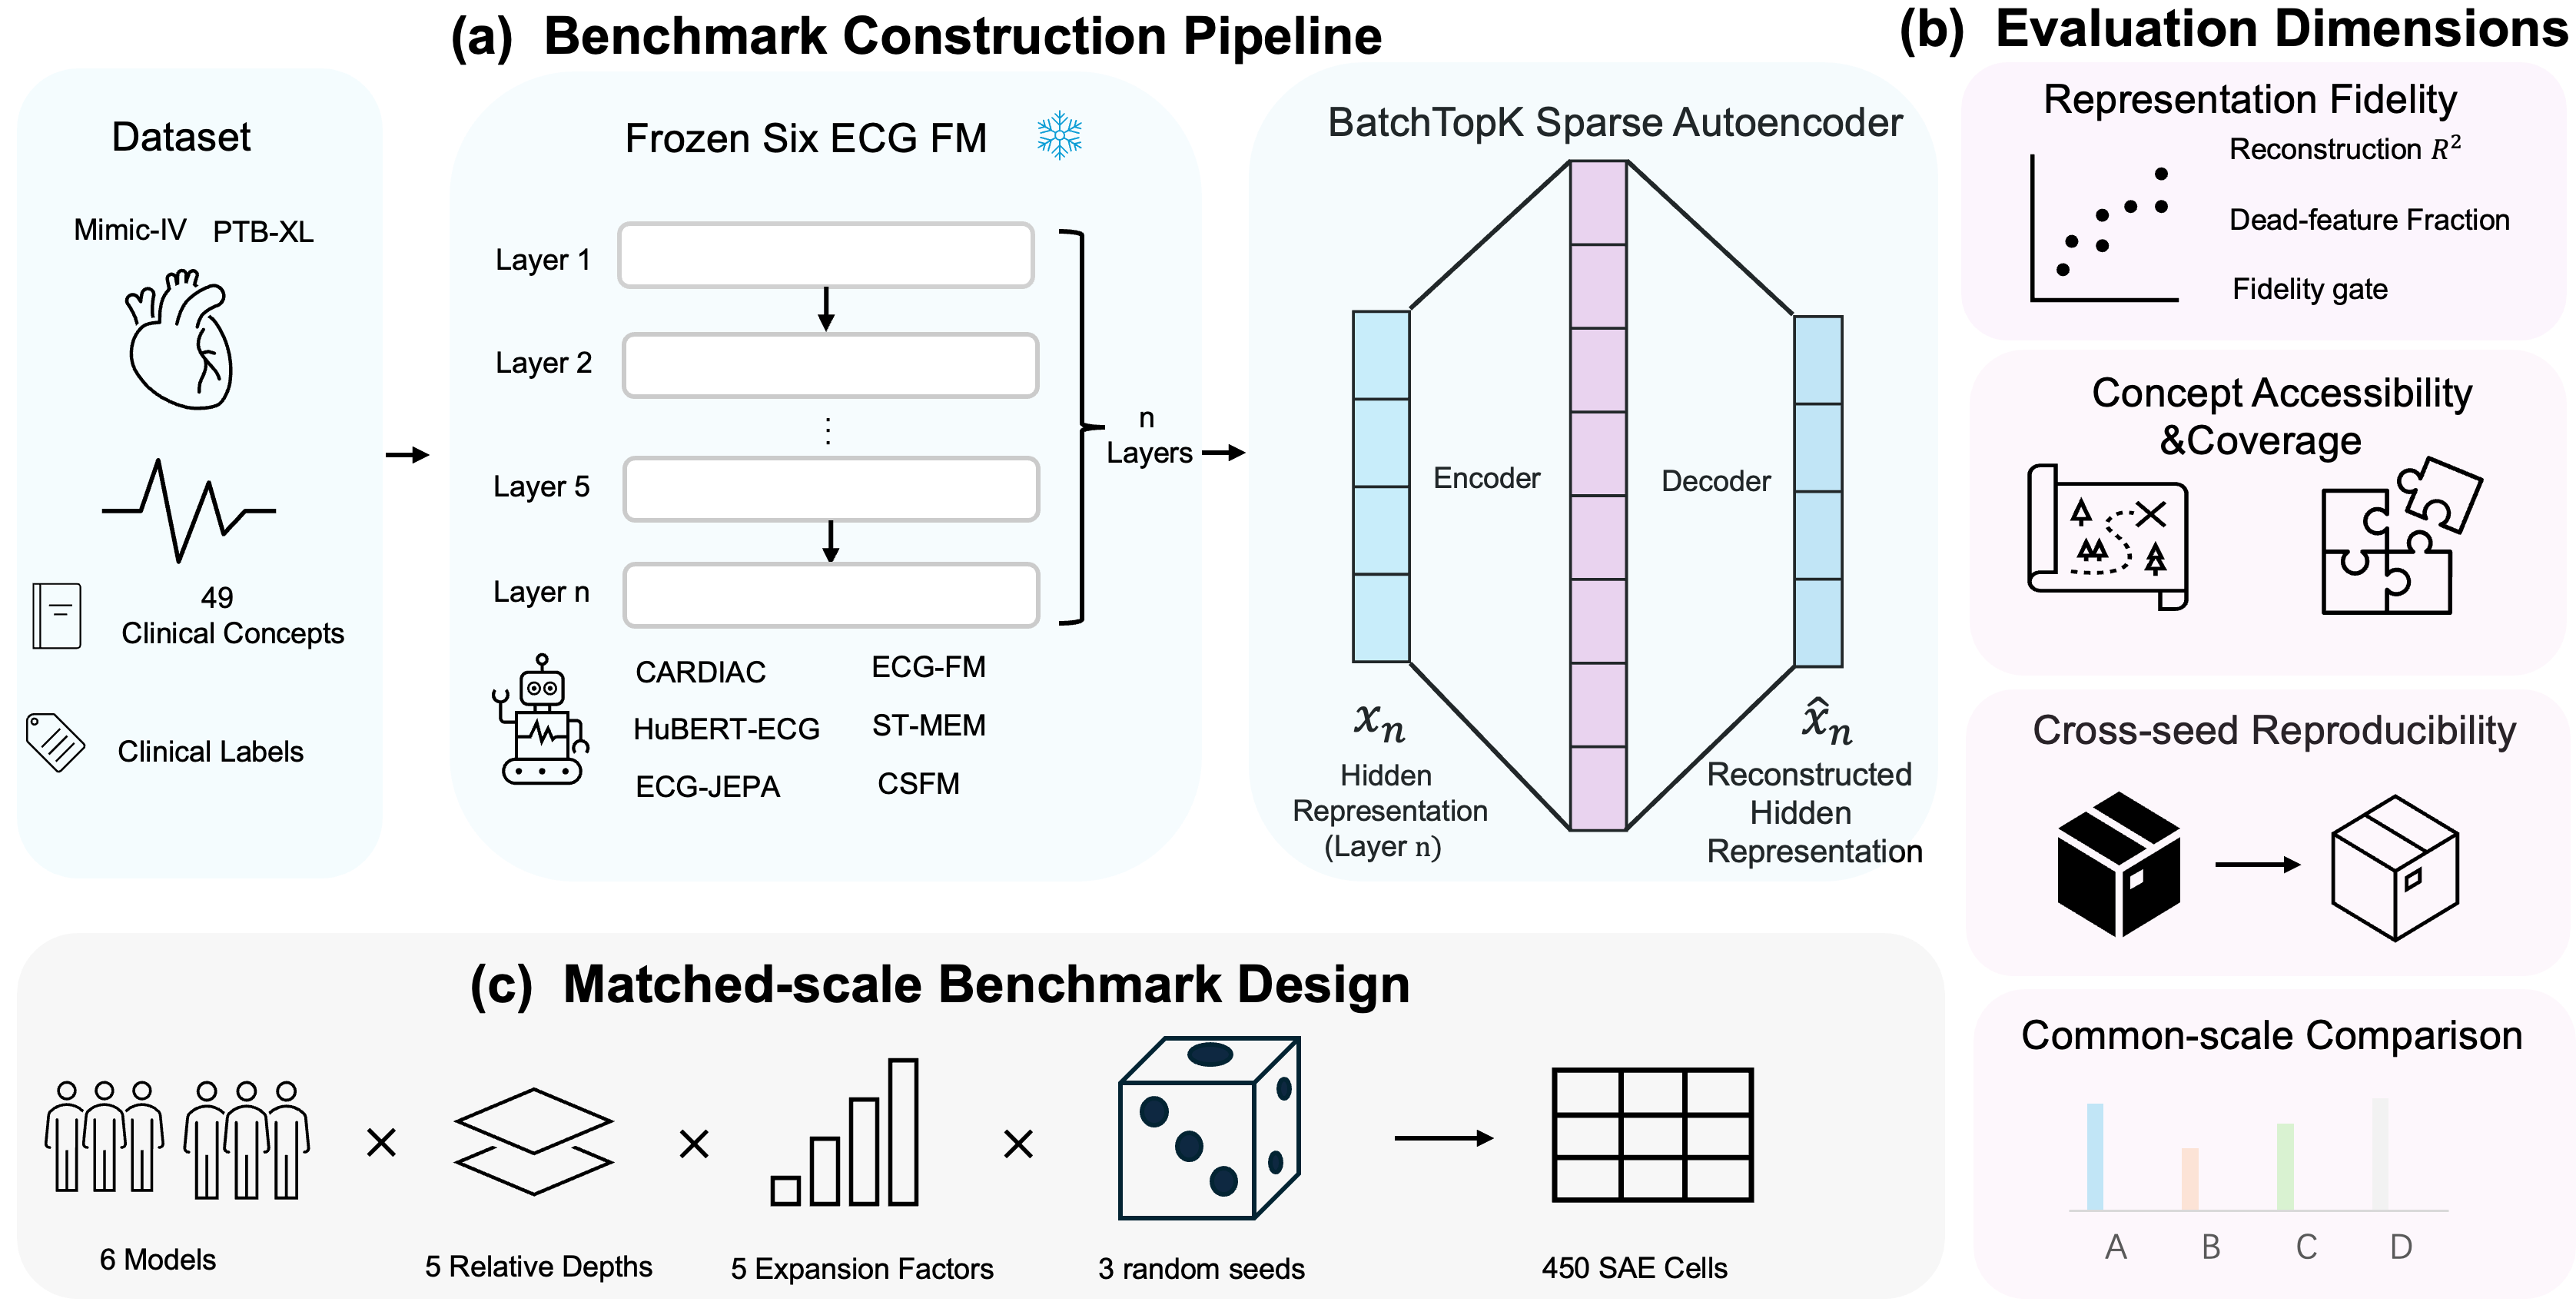
\includegraphics[width=\textwidth]{benchpipline.png}
  \caption{Overview of \bench. (a) PTB-XL and credentialed MIMIC-IV ECGs are passed through six frozen ECG FMs, and layer representations are decomposed with BatchTopK SAEs. (b) Each representation is evaluated separately for reconstruction fidelity, single-feature clinical concept accessibility and coverage, and cross-seed reproducibility. (c) The matched-scale design crosses six models, five relative depths, five expansion factors, and three seeds, producing 450 SAE cells for common-scale model comparison.}
  \Description{The benchmark pipeline has three parts. First, ECG datasets and clinical concepts are processed by six frozen ECG foundation models, and hidden representations from multiple layers are reconstructed by BatchTopK sparse autoencoders. Second, the resulting representations are evaluated for reconstruction fidelity, concept accessibility and coverage, and cross-seed reproducibility. Third, six models, five relative depths, five expansion factors, and three random seeds form a matched 450-cell comparison grid.}
  \label{fig:multiscale-workflow}
\end{figure*}

ECG foundation models (ECG FMs) learn general-purpose representations that support diverse rhythm, morphology, and cardiovascular risk-prediction tasks~\cite{mckeen2025ecgfm,gu2026csfm,na2024stmem}. Existing evaluations, however, focus primarily on downstream accuracy, transfer performance, or label efficiency~\cite{mehari2022ssl,kiyasseh2021clocs,vaid2023heartbeit}. These outcomes do not reveal how the hidden representation is organized: whether it can be faithfully decomposed, whether clinically relevant measurements are localized to identifiable features, or whether the same structure is recovered across independent decompositions. This gap matters in clinical settings because a shared representation can propagate acquisition artifacts, demographic confounding, or cohort-specific shortcuts to every downstream model built on it~\cite{rudin2019blackbox,ghassemi2021falsehope,tonekaboni2019clinicians}.

Existing interpretability tools address related but different questions. Output attribution identifies waveform regions that influence a prediction, but it does not audit the organization of a task-general hidden representation and may fail parameter-randomization or other sanity checks~\cite{strodthoff2019mi,adebayo2018sanity}. Linear probes establish whether a clinical variable is decodable, but not whether it is localized to a small number of features, preserved by a faithful sparse decomposition, or recovered across independent SAE trainings. Representation-level interpretability is therefore not equivalent to predictive accuracy, linear decodability, or visually plausible saliency; it requires explicit, complementary measurements~\cite{murdoch2019definitions}.

Sparse autoencoders (SAEs) provide a scalable instrument for this audit by mapping dense activations into sparse codes and reconstructing the original representation from learned decoder directions~\cite{cunningham2024sae,gao2025scaling,bussmann2024batchtopk}. Their behavior depends on dictionary width and sparsity, making capacity matching central to controlled cross-model measurement~\cite{templeton2024scaling,lieberum2024gemmascope,makelov2025principled}. \bench{} therefore evaluates every FM with the same family of dictionary scales and sparsity settings and summarizes all models over common scale support. This design separates differences among FM representations from differences in SAE measurement capacity.

\bench{} uses a matched family of SAEs as the standardized measurement instrument and treats the frozen FM representation as the object being evaluated. We operationalize representation interpretability along three separately reported axes: (1) sparse reconstruction fidelity and dictionary utilization; (2) train-selected single-feature accessibility and coverage of clinical ECG concepts; and (3) cross-seed reproducibility of decoder features and selected feature subspaces. Together, these axes provide a structured profile of how faithfully, locally, and reproducibly each representation can be interpreted.

We evaluate six frozen ECG FMs at five standardized relative depths, five matched SAE scales, and three random seeds. The resulting 450-cell atlas contains 75 comparison blocks in which all six models share the same target relative depth, dictionary capacity, sparsity protocol, and seed. Comparisons are made only within these blocks and summarized over the same scale support for every model. We additionally quantify patient-sampling and design uncertainty and test sensitivity to an alternative sparsity parameterization. Figure~\ref{fig:multiscale-workflow} summarizes this capacity-controlled design.

The benchmark reveals distinct, metric-specific interpretability profiles. Reconstruction fidelity, single-feature clinical accessibility, and decoder reproducibility expose complementary strengths across ECG FMs. A matched MIMIC-IV-ECG replication preserves the separation between reconstruction and accessibility leaders. The resulting profile supports direct model comparison across all measured representation properties.

Our contributions are:
\begin{itemize}[leftmargin=1.3em,itemsep=1pt,topsep=2pt]
  \item We introduce a capacity-controlled benchmark for comparing representation-level interpretability across six ECG FMs under a matched SAE protocol.
  \item We construct a 450-cell matched-scale interpretability atlas that maps how representation interpretability changes across encoder depth and SAE scale.
  \item We define leakage-controlled interpretability metrics spanning sparse fidelity, single-feature clinical accessibility and coverage, and cross-seed feature and subspace reproducibility.
  \item We provide robust interpretability comparisons supported by patient and design uncertainty, sparsity sensitivity, and external-cohort evaluation.
\end{itemize}
